\documentclass[aspectratio=169]{beamer}
\usepackage{luhmann}
\usepackage{tikz}
\usepackage{booktabs}

\title{secret gadget program}
\subtitle{q branch briefing}
\author{james bond \texttt{007}}
\date{\today}
\slidelink{https://mi6.gov.uk/briefings/gadgets}

\begin{document}

\frame{\titlepage}

\begin{frame}
    \frametitle{mission status}

    \begin{itemize}
    \item \textsb{Readiness level:} \al{greenlighted}
    \item \textsb{Mission risk:} \alr{elevated}
    \item \textsb{Backup protocol:} \alb{in testing phase}
    \end{itemize}

    \vspace{1em}

    \begin{wideitemize}
    \item \textsb{Active field agents:} 5
    \item \textsb{Undetected anomalies:} 2
    \item \textsb{Next sync with HQ:} \texttt{Friday 0700}
    \end{wideitemize}
\end{frame}

\begin{frame}
    \frametitle{gadget deployment matrix}

    \begin{tabular}{@{}lll@{}}
    \toprule
    \textbf{Gadget} & \textbf{Function} & \textbf{Status} \\
    \midrule
    DB12 & Off-road assault vehicle & \al{Operational} \\
    Omega Seamaster & EMP + decryptor & \alr{Faulty} \\
    Pen communicator & Long-range voice & \al{Operational} \\
    Cufflinks & Controlled detonation & \alb{Pending approval} \\
    Jetpack Mk II & Urban extraction & \alr{Unstable at altitude} \\
    \bottomrule
    \end{tabular}
\end{frame}

\begin{frame}
    \frametitle{schematic: pen communicator}

    \centering
    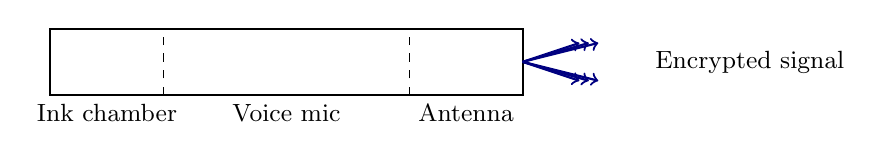
\begin{tikzpicture}[scale=1.2, every node/.style={font=\small}]
    % Pen body
    \draw[thick] (0,0) rectangle (5,0.7);
    % Sections
    \draw[dashed] (1.2,0) -- (1.2,0.7);
    \draw[dashed] (3.8,0) -- (3.8,0.7);
    
    % Labels
    \node[below] at (0.6,0) {Ink chamber};
    \node[below] at (2.5,0) {Voice mic};
    \node[below] at (4.4,0) {Antenna};

    % Waves
    \foreach \i in {0.1, 0.2, 0.3} {
        \draw[->, thick, NavyBlue] (5,0.35) -- ++(0.5+\i,0.2);
        \draw[->, thick, NavyBlue] (5,0.35) -- ++(0.5+\i,-0.2);
    }
    \node[right] at (6.3,0.35) {Encrypted signal};
    \end{tikzpicture}
\end{frame}

\lastslide

\end{document}
